\section{Results and Tests}

The testing of the energy consumption was done by measurement in the eAProfiler software.
While the program was running on the Development Board, some input was done, and the measurements was saved.

\subsection{Startup}

At the beginning of the program, a sound is played. 
As it's first the init code starting the sound, a step can be seen in the power consumption graph (figure \ref{fig:startuppower}).
\begin{figure}[H]
\centering
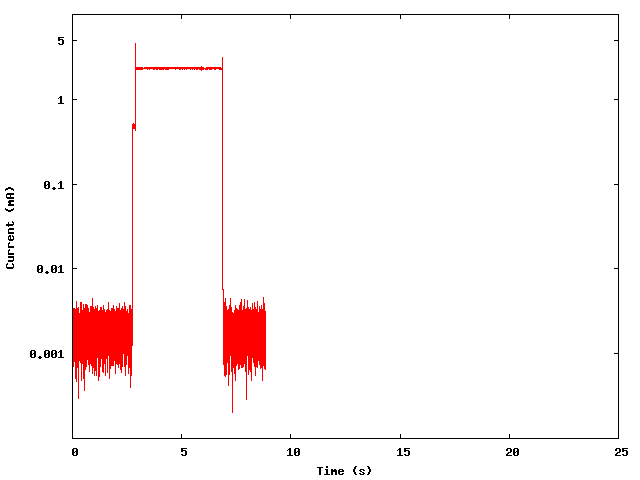
\includegraphics[width=0.75\textwidth]{data/startup.png}
\caption{Startup power consumption}
\label{fig:startuppower}
\end{figure}

\subsection{Playing music}
Figure \ref{fig:playpower} shows the power consumption of choosing a different song, and then playing that song.
It can be seen how the micro controller goes to sleep right after the button interrupt, and after the song is done playing.
Had DMA been implemented (see \vref{DMA}), the power consumption while playing sound would have been substansially lower.

\begin{figure}[H]
\centering
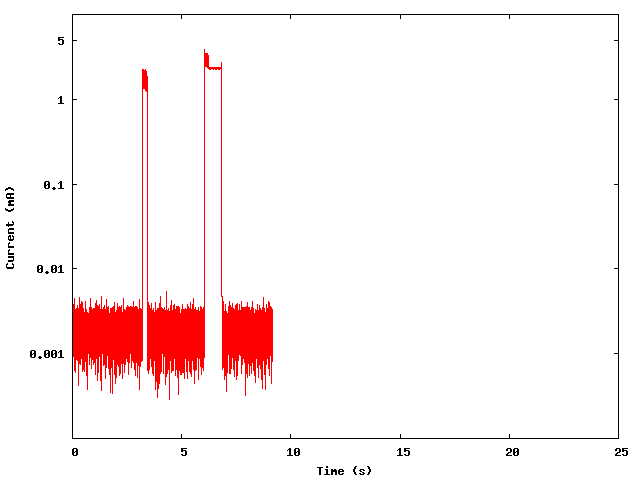
\includegraphics[width=0.75\textwidth]{data/play.png}
\caption{Playing power consumption}
\label{fig:playpower}
\end{figure}

\subsection{Holding}
When holding down a button, a peculiar pattern emerges (see figure \ref{fig:holdingpower}). 
Theres a spike at first, and then a lower energy level.
This is because as a button is pressed, the circuit being first closed will generate more power.
While not a wanted feature, there's is nothing to do about this.

\begin{figure}[H]
\centering
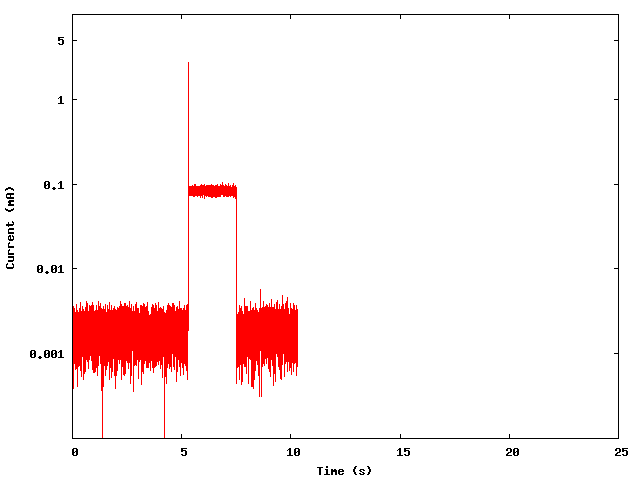
\includegraphics[width=0.75\textwidth]{data/hold.png}
\caption{Power consumption while holding button}
\label{fig:holdingpower}
\end{figure}
